\documentclass[twocolumn]{aastex631}

% Packages
\usepackage{microtype}  % ALWAYS!
\usepackage{amsmath}
\usepackage{amsfonts}
\usepackage{amssymb}
\usepackage{multirow}
\usepackage{tikz}
\usepackage{xcolor}
\usepackage{soul}

\definecolor{pink}{RGB}{232,132,161}
\definecolor{yellow}{RGB}{255,213,0}

\newcommand{\kc}[1]{\textcolor{yellow}{\textbf{kc: #1}} }
\newcommand\shadetext[2][]{%
  \setbox0=\hbox{{\special{pdf:literal 7 Tr }#2}}%
  \tikz[baseline=0]\path [#1] \pgfextra{\rlap{\copy0}} (0,-\dp0) rectangle (\wd0,\ht0);% 
  }
\newcommand{\gb}[1]{\shadetext[left color=blue, right color=red, middle color=lime, shading angle=45]{\textbf{g: #1}} }
% \newcommand{\ecite}[1]{\textcolor{pink}{\textbf{: #1}} }
% \newcommand{\e}[1]{\textcolor{yellow}{\textbf{: #1}} }

\newcommand{\remove}[1]{\textcolor{red}{#1}}
\newcommand{\add}[1]{\textcolor{green}{#1}}

\newcommand{\mlg}{\ensuremath{M_{\rm LG}}}
\newcommand{\mmto}{\ensuremath{M_{\rm M31}}}
\newcommand{\mmw}{\ensuremath{M_{\rm MW}}}
\newcommand{\vtan}{\ensuremath{v_\textrm{tan}}}
\newcommand{\vrad}{\ensuremath{v_\textrm{rad}}}
\newcommand{\ms}[1]{\ensuremath{M_{*{#1}}}}
\newcommand{\mud}{\ensuremath{\mu_\delta}}
\newcommand{\mua}{\ensuremath{\mu_\alpha^*}}
\newcommand{\bov}{\ensuremath{\boldsymbol{v}}}
\newcommand{\boldx}{\ensuremath{\boldsymbol{x}}}
\newcommand{\vtrav}{\ensuremath{\bov_{\rm travel}}}
\newcommand{\xtrav}{\ensuremath{\boldx_{\rm travel}}}
\newcommand{\pos}[2]{\ensuremath{\boldx_{\rm #1 \to #2}}}
\newcommand{\vel}[2]{\ensuremath{\bov_{\rm #1 \to #2}}}
\newcommand{\mwbary}{\ensuremath{\textrm{MW}_\textrm{bary}}}
\newcommand{\mwouter}{\ensuremath{\textrm{MW}_\textrm{halo}}}
\newcommand{\mwdisk}{\ensuremath{\textrm{MW}_\textrm{disk}}}
\newcommand{\reflabel}[1]{\ensuremath{^{\mbox{\scriptsize{#1}}}}}
\newcommand{\scsep}{\ensuremath{\rm r_{sep}/r_{vir}}}
\newcommand{\scvel}{\ensuremath{\rm v_{rel}/v_{vir}}}

% Style tweaks
% \renewcommand{\twocolumngrid}{\onecolumngrid}
% \setlength{\parindent}{1.1\baselineskip}
% \sloppy\sloppypar\raggedbottom\frenchspacing

%%%%%%%%%%%%%%%%%%%%%%%%%%%%%%%%%%%%%%%%%%%%%%%%%%%%%%%%%%%%%%%%%%%%%%%%%%%%%%%%
\shorttitle{Frequency of galaxy pairs}
\shortauthors{Chamberlain et al.}

%%%%%%%%%%%%%%%%%%%%%%%%%%%%%%%%%%%%%%%%%%%%%%%%%%%%%%%%%%%%%%%%%%%%%%%%%%%%%%%%
\graphicspath{{./}{../plots/paper1/}}
% Missions
\newcommand{\project}[1]{\textsl{#1}}

% Packages / projects / programming
\newcommand{\package}[1]{\textsl{#1}}
\newcommand{\acronym}[1]{{\small{#1}}}
\newcommand{\github}{\package{GitHub}}
\newcommand{\python}{\package{Python}}
\newcommand{\astropy}{\package{Astropy}}

% Stats / probability
\newcommand{\given}{\,|\,}
\newcommand{\norm}{\mathcal{N}}
\newcommand{\pdf}{\textsl{pdf}}

% Maths
\newcommand{\dd}{\mathrm{d}}
\newcommand{\transpose}[1]{{#1}^{\mathsf{T}}}
\newcommand{\inverse}[1]{{#1}^{-1}}
\newcommand{\argmin}{\operatornamewithlimits{argmin}}
\newcommand{\mean}[1]{\left< #1 \right>}

% Non-scalar variables
\renewcommand{\vec}[1]{\ensuremath{\bs{#1}}}
\newcommand{\mat}[1]{\ensuremath{\mathbf{#1}}}

% Unit shortcuts
\newcommand{\Msun}{\ensuremath{\mathrm{M}_\odot}}
\newcommand{\Mjup}{\ensuremath{\mathrm{M}_{\mathrm{J}}}}
\newcommand{\kms}{\ensuremath{\mathrm{km}~\mathrm{s}^{-1}}}
\newcommand{\pc}{\ensuremath{\mathrm{pc}}}
\newcommand{\kpc}{\ensuremath{\mathrm{kpc}}}
\newcommand{\Mpc}{\ensuremath{\mathrm{Mpc}}}
\newcommand{\kmskpc}{\ensuremath{\mathrm{km}~\mathrm{s}^{-1}~\mathrm{kpc}^{-1}}}
\newcommand{\dayd}{\ensuremath{\mathrm{d}}}
\newcommand{\yr}{\ensuremath{\mathrm{yr}}}
\newcommand{\Myr}{\ensuremath{\mathrm{Myr}}}
\newcommand{\Gyr}{\ensuremath{\mathrm{Gyr}}}
\newcommand{\Kel}{\ensuremath{\mathrm{K}}}
\newcommand{\masyr}{\ensuremath{\mathrm{mas}~\mathrm{yr}^{-1}}}
\newcommand{\muasyr}{\ensuremath{\mu\mathrm{as}~\mathrm{yr}^{-1}}}

% Misc.
\newcommand{\bs}[1]{\boldsymbol{#1}}

% Astronomy
\newcommand{\DM}{{\rm DM}}
\newcommand{\feh}{\ensuremath{{[{\rm Fe}/{\rm H}]}}}
\newcommand{\df}{\acronym{DF}}

% TO DO
\newcommand{\todo}[1]{{\color{red} TODO: #1}}
\newcommand{\apw}[1]{{\color{blue} APW says: #1}}

% Projects
\newcommand{\gaia}{\textsl{Gaia}}
\newcommand{\gaiadr}{\textsl{Gaia}~\acronym{EDR3}}
\newcommand{\hst}{\textsl{HST}}
\newcommand{\ill}{\textsl{Illustris}}
\newcommand{\tng}{\textsl{IllustrisTNG}} 



% Affiliations
\newcommand{\affuofa}{University of Arizona, 933 N. Cherry Ave,
    Tucson, AZ 85721, USA}

%% This is the end of the preamble.  Indicate the beginning of the
%% manuscript itself with \begin{document}.

\begin{document}

\title{
  Frequency of dwarf and massive galaxy pairs in the IllustrisTNG cosmological simulation
}

\author[0000-0001-8765-8670]{Katie~Chamberlain}
\affiliation{\affuofa}

\author[0000-0003-0715-2173]{Gurtina Besla}
\affiliation{\affuofa}


\begin{abstract}
  
  \todo{Remove all instances of "we find" to "we compute" or "we calculate"}
\end{abstract}

%%%%%%%%%%%%%%%%%%%%%%%%%%%%%%%%%%%
\section{Introduction} \label{sec:intro}


%%%%%%%%%%%%%%%%%%%%%%%%%%%%%%%%%%%
%%%%%%%%%%%%%%%%%%%%%%%%%%%%%%%%%%%
 \section{Methodology}\label{sec:methods}
We aim to quantify and characterize the frequency (or occurrence rate) and bulk kinematic properties of galaxy pairs in a cosmologically consistent way a function of cosmic time. 
In particular, we study dwarf galaxy pairs and massive galaxy pairs that are of similar stellar and halo mass to a variety of pairs in the Local Group. 
We categorize these pairs into one of four pair types: massive major pairs, such as the MW+M31; massive minor pairs, such as M31+M33 or MW+LMC; dwarf major pairs, such as M33+LMC; and finally, dwarf minor pairs, such as the LMC+SMC. 

To this end, we use a run of the \tngh\ simulation to select halo pairs at each snapshot according to a strict set of selection criteria as outlined in the remainder of this section. 
In Sec.~\ref{sec:methods-sims}, we provide motivation for and details of the simulation utilized in this study.
Sec.~\ref{sec:methods-halos} outlines the initial mass cuts used to define our full sample of halos, from which we will select pairs.
Sec.~\ref{sec:methods-am} outlines the abundance matching prescription we used to associate dark matter subhalos with stellar masses.
Sec.~\ref{sec:methods-pairs} describes the second set of selection criteria we apply to obtain the full sample of pairs.
In Sec.~\ref{sec:methods-props}, we show some of the properties of our entire pair sample, including the total number of pairs and stellar mass ratios.
Finally, Sec.~\ref{sec:methods-analysis} gives an overview of our analysis methods and a description of the parameters of interest in this study. 

%%%%%%%%%%%%%%%%%%%%%%%
% Sim details section %
    \subsection{Simulation details} \label{sec:methods-sims}
        % Brief description of TNG hydro and which run we use.
    The \tng\ project ~\citep{TNG1, TNG2, TNG3, TNG4, TNG5} consists of a suite of dark-matter-only $N$-body as well as full physics cosmological simulations consistent with the \textit{Planck2015} \lcdm/  cosmology~\citep{Planck2015}.
    In this study we utilize data from the main high resolution full physics run of the (110.7\Mpc)$^3$ volume simulation, \textsl{TNG100-1}, which includes dark matter and baryonic particles and follows the evolution of $1820^3$ dark matter particles in 100 snapshots from $z=127$ to $z=0$. 

      % subfind, sublink, and groups and subhalos
    We utilize the group catalogs produced by the \texttt{SUBFIND} algorithm~\citep{springel2001,dolag09}. 
    These catalogs consist of halos , defined using the Friends-of-Friends (FoF) algorithm~\citep{davis1985} to link nearby particles, and their associated subhalos, which are over-dense and gravitationally bound dark matter structures compared to the background. (From here, we will refer to FoF halos as "groups" and their subhalos as )
      % We also use merger catalogs generated by XX for YY purpose. 
    We also use merger trees provided by the \texttt{SUBLINK} algorithm~\citep{RG2015}, which tracks subhalos between snapshots using their DM particle data, in order to trace subhalo mass growth and merger histories.
    
    The large volume of this simulation offers a large statistical sample of halos to study in a cosmological context, but is also high enough resolution ($m_{\rm DM} = 7.5\times10^6\Msun$, $m_{\rm gas} = 1.4\times10^6\Msun$) that dwarf halos ($\sim1\times10^{9-10.5}\Msun$) halos are resolved into roughly hundreds or more particles, well above the resolution limit of 32 DM particles for halos identified with \texttt{SUBFIND}, and 20 gas and star particles used to construct baryonic merger trees.  

        %  this MIGHT go in a different section? am I talking about this because I want to show why we use hydro instead of dark? 
    Baryonic process are known to affect the structure and formation of dark matter halos of low mass ($M_*\lesssim 1\times10^9\Msun$) subhalos in simulations~\citep[see e.g.][and references therein]{Sales:2022}.
    Additionally, the shallow potential well of dwarf galaxies compared to their massive counterparts may lend themselves more easily to disruption from baryonic processes such as supernova feedback and reionization~\citep{}, resulting in fewer low mass halos ($\lesssim 5\times10^{10}$) in hydrodynamic simulations~\citep{vogelsberger14B}.
    % Thus, the number of primaries  we expect that our choice of simulation will result in 
% End sim details     %
%%%%%%%%%%%%%%%%%%%%%%%

%%%%%%%%%%%%%%%%%%%%%%%%%%    
% Choosing halos section %
    \subsection{Choosing dwarf and massive halos in TNG} \label{sec:methods-halos}
    % start off with group selection 
        % brief explanation of FoF groups in sim
    Each snapshot from the TNG100 group catalogs consist of FoF groups, large halos of closely associated DM particles, and the subhalos they contain, which are smaller bound structures of DM and the gas and star particles nearest to them. 
    We will refer to these two structures as "groups" and either "halos" or "subhalos" respectively, from here on. 
    Galaxies form in these subhalos, so our pair sample will consist of pairs of subhalos within these larger group structures.

    We are interested in the inherent dynamics and properties of pairs of halos in the field.
    Thus, we want our pairs to consist of some of the most massive halos in each group, and ensure that the pair is not dynamically influenced by nearby massive groups. 
    By selecting pairs from the most massive halos of a group, a rough isolation criteria is inherent in our selection due to the nature of the FoF algorithm, which groups together nearby particles. 
    To confirm that our sample , we have confirmed that nearly 100\% of the the most massive subhalos in each group are outside of the Hill radius of any nearby group or subhalo with greater mass.

    The first selection criteria that we invoke is a cut on the total group mass, $M_{G}$ (i.e., a mass cut on the FoF group mass, given by \texttt{Group\_M\_TopHat200} in the \tng\ group catalogs). 
    We define the group mass range for dwarf groups as $8\times 10^{10} < M_{G,d} < 5\times 10^{11}\Msun$, which will host mass analogs of the LMC+SMC and LMC+M33 pairs. 
    Massive group a massive group mass range from $1\times10^{12} < M_{G,m} < 6.5\times10^{12}$, which at the lower mass end will host MW+LMC pairs, and MW+M31 pairs at the higher mass end. 
    The group mass criteria is fixed for all redshifts, so at high z, the dwarf pairs we select may be the progenitors of higher mass systems at $z=0$.
    Note that all masses used in this analysis are physical units, such that masses from the group catalogs are divided by $h$ to get units of \Msun. 

    Selecting dwarf pairs from the dwarf group mass range also ensures that we are not selecting satellite systems in the halos of more massive systems. 
    The LMC+SMC, for example, are highly perturbed by the influence of the MW, and thus we do not pick dwarf pairs from high mass groups that may contain large nearby MW-mass analogs.
    
        % explain what halos we will move forward with. 
    For each group that passes the group mass cut, we create a catalog of all subhalos that pass a ``current mass" criteria: current (same snapshot) halo mass must be $M_h > 1\times10^{9}\Msun$ (the \texttt{SubhaloMass} field in the group catalogs).\footnote{Note that for the TNG100 hydro run, the halo mass is the total sum of all bound dark matter \textit{and} baryonic particles.}
    This lower mass threshold ensures that our halos are resolved into $>100$ particles, and thus should be robust to the SUBFIND and SUBLINK algorithms even at the lowest mass end.  
    
    We then utilize the merger tree catalogs to determine the maximum halo mass ever achieved by each halo. 
    The set of all subhalos at each snapshot that pass the group mass and current mass cuts constitutes our entire subhalo sample. 
    From here, we will use further selection criteria to narrow our sample down to pairs.

% End choosing halos     %
%%%%%%%%%%%%%%%%%%%%%%%%%%    


%%%%%%%%%%%%%%%%%%%%%%%%%%    
% Choosing halos section %
    \subsection{Abundance matching} \label{sec:methods-am}
        % what is abundance matching
    Abundance matching is a technique used to associate dark matter halo mass with specific galaxy properties.
    This allows us to associate dark matter halos from the \tng\ simulation with observationally motivated galaxy properties. % maybe observationally constrained, instead? 
    In particular, we will be utilizing a stellar mass to halo mass (SMHM) relationship to assign stellar masses to each of the subhalos in our sample. 

    % few details about the msoter relationship. how was it determined?
        % why are we using abundance matching 
    The \tng100-1 subhalo catalogs do already contain a stellar mass field as computed in the simulation by simulating star formation and  AGN feedback, stellar feedback, galactic winds, etc.    
    However, there are a couple reasons we opt to assign stellar masses to our halos, rather than use those from the simulation. 
    
    Primarily, applying an abundance matching prescription to assign stellar masses to each of the dark matter halos allows us to account for the observed spread in the stellar mass-halo mass relationship. 
    This is particularly important in the low mass regime ($M_h \lesssim 10^{11}\Msun$) where the spread in the SMHM function is large. 
    In addition, using stellar masses as calculated from abundance matching allows us to side step any simulation-dependent stellar mass effects.
    In the case of \tng100 specifically, it is known that the stellar masses of low mass galaxies are often overestimated compared to the galaxy luminosity function at the low mass end\cite{}. 
    Using an observationally-calibrated abundance matching prescription will thus lead to a more robust result for comparison with and predictions for observations. 
    Finally, utilizing an abundance matching prescription allows us to directly compare results between dark matter only and hydro simulations, since the stellar masses are assigned the same way. 
    We make brief note of results from dark matter only simulations in Sec.~\ref{sec:results}.
    
        % what am prescription are we using? 
    We use the abundance matching relationship presented in~\citet{Moster2013}, which provides an analytic recipe to assign stellar masses to dark matter halos. 
    The~\citet{Moster2013} relationship is a function of the halo mass, evolves with redshift, and includes terms to account for the systematic scatter in the SMHM relationship, with larger scatter at lower halo masses.
    Additionally, stellar mass is defined separately for central halos (``hosts") and for infalling satellites (``subhalos"), where the first is a function of the virial mass of the halo and its redshift, $M_{vir}$ and $z$, and the second is a function of the mass and redshift at the time of infall, $M_{inf}$ and $z_{inf}$. 
    This assumes that the satellite halos are at the peak of their stellar mass before infall, and neglects the affect of star formation or stellar stripping within the host halo. 

        % what do we use for the mass ~ 
    In this work, we will use the peak halo mass \Mpeak\ from the \sublink\ merger trees to calculate subhalo stellar masses. 
    \citet{Munshi2021} found that the stellar mass of subhalos at $z=0$ in the ``Marvel-ous Dwarfs" and ``DC Justice League" zoom simulations are more closely correlated with the peak halo mass ($M_{peak}$) than the $z=0$ halo mass for halos with peak halo mass $10^8<M_{\rm peak}<10^{11} \Msun$. 
    % separate citation for peak halo mass and stellar mass relatiosnhip for M > 1e11Msun 
    Using the peak halo mass additionally allows us to remain robust to scenarios in which a secondary has formed most of its stars, then loses a significant portion of its dark matter content through tidal interactions with a primary, but retains the bulk of its stellar content.
        
        % regarding the redshift dependence ~
    We additionally assume that the stellar mass of both the primary and secondary halo can change as a function of redshift after the secondary has entered the primary's halo and do not immediately cease star formation. 
    This assumption is consistent with findings from~\cite{Akins2021}, which found that massive dwarf satellites ($M_*\approx 10^8-10^9\, \Msun$) entering MW-mass host halos are rarely quenched, and with~\cite{geha13} which finds that dwarfs $>1\Mpc$ from a MW-type galaxy are often star forming and rarely quenched.
    Additionally, the SAGA survey has found that large satellites of MW-type galaxies are often very blue, with infall into the halo spurring high rates of star formation due to the large gas fraction in dwarfs~\citep{saga}. 
    Thus, we calculate stellar masses for our subhalos using $M_{\rm peak}$ and the redshift of the current snapshot to calculate the stellar mass of each subhalo, to account for the additional stellar mass that can form after infall. 

    As mentioned in a footnote in Sec.~\ref{sec:methods-halos}, the total halo mass of subhalos in the hydro simulation includes the mass of both dark matter and baryonic particles. 
    In TNG100-1, the DM particle mass is decreased XX\% compared to the DM particle mass in \tng100-1 Dark to account for the additional mass of baryons, such that the total mass of the halo will remain roughly the same between the dark matter only and hydro simulations. 
    Since the~\citet{Moster2013} AM relation was calibrated using DM subhalos from the \texttt{MilleniumII} dark matter only simulation, we will use the total subhalo mass from the TNG100-1 hydro simulation as a proxy for the corresponding DM halo mass in the TNG100-1 Dark run. 

        % realizations? 
    For each subhalo at each snapshot in our full subhalo sample (see Sec.~\ref{sec:methods-halos}), we create a set of 1000 stellar mass values from the SMHM relationship to account for the systematic uncertainty in subhalo stellar masses.
    Each realization is treated as an independent sample of galaxy stellar masses, which allows us to report realistic spreads of pair properties.
    Thus, we create 1000 separate pair catalogs, and compute pair properties (pair frequency, separations, etc) for each individual abundance matching realization.

% End choosing halos     %
%%%%%%%%%%%%%%%%%%%%%%%%%%      

%%%%%%%%%%%%%%%%%%%%%%%%%%    
% Pair selection section %
    \subsection{Pair selection}\label{sec:methods-pairs}
    The full pair sample is constructed from the set of all subhalos and their abundance matching realizations. Each pair will consist of a ``primary" more massive object, and a ``secondary" less massive companion. 

    % justify why we want to use stellar mass to define things
    A majority of the literature uses the definition of "major" and "minor" pairs based on the stellar mass of the objects. This is true as well for observational pair samples, such as Lotz 2011, wherein the halo mass of the objects is unknown, and thus the stellar mass is used to define the mass ratio of the pair. In order to reproduce statistics that can be meaningfully compared to observations/can be used to inform observations, we opt to define our pair sample via the stellar masses from the abundance matching prescription given in Sec.~\ref{sec:methods-am}. 

    %%% 
    % begin subsubsection
    \subsubsection{Selecting primaries}
    Primary galaxies (equivalently, ``primary subhalos") are the most massive galaxy of their group by stellar mass. Thus, each group can have at most one primary galaxy.  
    
    We perform mass cuts on the stellar mass of the primary to define our sample of dwarf primaries and massive primaries. Each stellar mass realization is treated independently, such that the primary of a group may change between stellar mass realizations. Additionally, some groups may not have a ``primary" in one realization, but will in others. 

    For each stellar mass realization, we rank order the subhalos of each group by stellar mass, then perform a mass cut specific to the type of group: dwarf primaries from dwarf mass groups, and massive primaries from massive mass groups (see Sec.~\ref{sec:methods-halos} for group mass criteria). 
    We define the stellar mass range for dwarf primaries and massive primaries as:
    \begin{align*} 
    \mbox{\textbf{dwarf primaries:}}&\, 1\times 10^{8}< \rm M_{*} < 5\times10^{9}\Msun \\ 
    \mbox{\textbf{massive primaries:}}&\, 5\times 10^{9}< \rm M_{*} < 1\times 10^{11}\Msun.
    \end{align*}
    
    The stellar mass criteria is fixed, and does not change as a function of redshift. 
    The median number of primaries in a single stellar mass realization at $z=0$ is XX dwarf primaries and XX massive primaries (see Sec.~\ref{sec:methods-props} for more info). 
    The primary stellar mass range is chosen to replicate a set of pairs with masses similar to LMC+SMC and MW-M31. 
    
    The abundance matching prescription has a spread of $\sim 1$dex at $M_{h}\sim 10^{10}\Msun$~\citep{Moster2013}, thus the set of selected primaries in each realization is typically unique. 

    % explain special cases that people might wonder about.
    A subhalo will not be selected as a primary if it is not the first most massive halo in the group, i.e., there are no subhalos in the group that are more massive than the primary (by stellar mass). However, since our selection is based on stellar mass, and there is a large spread in the SMHM relation, the most massive object by stellar mass may not be the most massive subhalo in terms of subhalo mass. 
    This is by design, since our selection criteria are meant to more closely replicate observational pair selection criteria which use the stellar mass ratio between the primary and companion to define a major or minor pair, rather than the DM halo mass. 

    If a subhalo passes the stellar mass cut for a primary, but does not have an associated companion from the selection criteria for a secondary (see next subsection), the subhalo will still be considered a primary. We refer to all primaries without companions as ``isolated primaries."
    The total set of primaries includes both paired primaries and isolated primaries.
    % end  primary subsubsection
    %%% 
    
    %%% 
    % begin secondary subsubsection
    \subsubsection{Selecting secondary companions}
    The second most massive galaxy by stellar mass in each group is then used to define the secondary companions for each primary. 
    As before, the selection of secondary companions occurs independently for each stellar mass realization, and for each snapshot, such that we collect 1000 different sets of pairs for each redshift.
    
    We create two categories of pairs: 
    major pairs and minor pairs, such that the secondary companion galaxies are selected via the stellar mass ratio between the secondary and primary.     
    Since we have already rank ordered the halos in each stellar mass realization by their stellar mass, the stellar mass ratio will never exceed 1.   
    The stellar mass ratio criteria for major and minor pairs are:
    \begin{align*} 
    \mbox{\textbf{major pair:}}&\, \frac{1}{4}\leq \frac{\rm M_{*2}}{\rm M_{*1}}< 1 \\ 
    \mbox{\textbf{minor pair:}}&\, \frac{1}{10}\leq \frac{\rm M_{*2}}{\rm M_{*1}} < \frac{1}{4}
    \end{align*}
    In addition, we require that each pair have a minimum separation of $15\kpc$ between the primary and secondary, which is XX times the smoothing length of the simulation. 
    At smaller separations, more and more mass will be attributed to the central subhalo, which can lead to confusion in the merger tree histories. \kc{fix the wording here}.
  
    If a primary subhalo does not have a companion that meets the stellar mass ratio criteria, separation criteria, or lower subhalo mass criteria (see Sec.~\ref{sec:methods-halos}), the subhalo will still be considered a primary. 
    We refer to all primaries without companions as ``isolated primaries."

    Note that in this selection routine, the LMC+SMC pair would not be selected, as they are a system of satellites in a massive group. Rather, the MW-M31 pair would be selected and identified as a ``massive major pair."
    % end secondary subsubsection
    %%% 
    
% Pair selection end %
%%%%%%%%%%%%%%%%%%%%%%

%%%%%%%%%%%%%%%%%%%%
% Pair prop. start %
    \subsection{Overview of selected pair sample} \label{sec:methods-props}
        The full pair sample contains 1000 individual sets of pairs at each snapshot, for all 100 snapshots of the \tng100-1 simulation. 
        For each snapshot, we calculate the median number of primaries and pairs in each of the 1000 stellar mass realizations. 
        The data shown is the median and 1-99\% range of the set of medians from the realizations.
    
        Fig.~\ref{fig:counts} shows the redshift evolution of the number of dwarf and massive primaries and pairs we identify over the redshift range $z=0-4$. 
        The number of identified primaries is smallest at $z=4$, and rises to a maximum around $z=1$ for both dwarf and massive primaries.        
        There are approximately 8 times as many dwarf primaries as massive primaries. 
        
        The dwarf primary count (green solid line in top left panel) reaches a maximum median of $\sim15000$ halos (in one realization) at $z\sim0.6$, then decreases by $\sim16\%$ to 12000 halos at $z=0$. 
        The dwarf pair count (green dashed line) peaks much earlier at $z\sim2$ with $\sim3000$ pairs, and decreases to $\sim1000$ pairs at $z=0$.
        The massive primary count (pink solid line in top right panel) reaches a maximum median of $\sim2000$ halos (in one realization) at $z\sim1$, then remains approximately constant to $z=0$. 
        The pair count for massive galaxies (pink dashed line) behaves similarly to the primary count, increasing from $z=4$ to $z\sim1$, then leveling off to $z=0$.

        The bottom panel of Fig.~\ref{fig:counts} shows the number of pairs divided by the number of primaries, or the fraction of pairs per primary as a function of redshift. 
        Dwarf and massive pair fractions are roughly flat for $z=2.5-4$, but display opposite behavior for $z=0-2.5$. The dwarf pair fraction decreases steadily from $\sim0.24$ to $\sim0.08$, a decrease of roughly $65\%$, while the massive pair fraction is roughly flat between $z=1-2.5$ with an average of $0.31$, before spiking sharply from $\sim 0.29$ to $\sim 0.36$ between $z=0-0.25$, an increase of $25\%$.

        We show the distribution of stellar mass ratios between the secondary and primary of each dwarf and massive pair in Fig.~\ref{fig:massratio}.
        % Major pairs make up $51-55\%$ of the full sample of pairs at every redshift for both dwarf and massive pairs.
        In general, the shape of the distribution remains constant from $z=0-4$ for both dwarfs and massive pairs, and between the dwarf and massive pairs at each redshift. 
        Thus, the typical stellar mass ratio of pairs in our sample is independent of mass scale and of redshift.


            
% Pair prop. end %
%%%%%%%%%%%%%%%%%%

%%%%%%%%%%%%%%%%%%%%%%
% begin method plots %
  \begin{figure*}[htp]
    \centering
    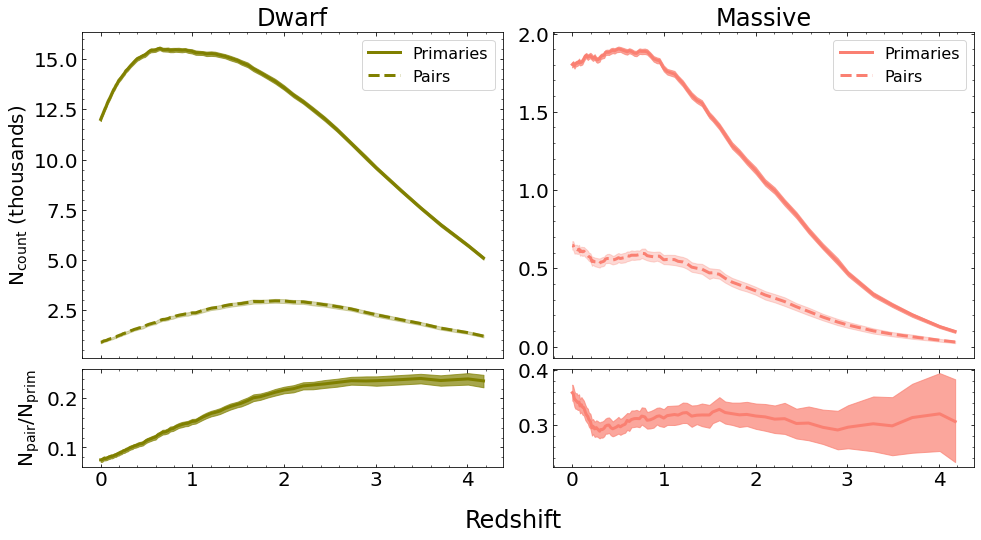
\includegraphics[width=\textwidth]{counts_1000.png}
    \caption{(Top) Median number of dwarf (left) and massive (right) primaries and pairs as a function of redshift.
    Shaded areas show the 1-99 percentile range of the median from 1000 abundance matching realizations, as described in Sec.~\ref{sec:methods-err}.
    There are approximately 8 times as many dwarf primaries as massive primaries. 
    % dwarf galaxies
    The dwarf primary count (solid) is at a minimum at $z=4$, rises to a maximum by $z\sim1$, then decreases from $z=1\to0$. 
    The dwarf pair count (dashed) peaks at $z\sim2$.
    % Massive galaxies (right)
    The massive primary count (pink solid line in top right panel) behaves similarly to the dwarf primary count, with a minimum count at $z=4$ which rises to a maximum of $\sim2000$ halos per realization at $z\sim1$, then decreases slightly by $\sim5\%$ to $\sim$1800 halos by $z=0$. 
    Unlike dwarf pairs whose pair count peaks at $z=2$, pair count for massive galaxies (pink dashed line) follows similar behavior to the total massive primary count, with a minimum at $z=4$, and increasing to $z=\sim 1$ before leveling off. At very low redshift, the pair count and primary count have opposite behavior, with the pair count \textit{increasing} at very low redshifts of $z=0-0.25$ and \textit{peaking} at $z=0$.
    (Bottom) Fraction of pairs per primary as a function of redshift (i.e., the ratio between dotted line and solid line in each column). Dwarf and massive pair fractions are roughly flat for $z=2.5-4$, but display opposite behavior for $z=0-2.5$. The dwarf pair fraction decreases steadily from $\sim0.24$ to $\sim0.08$, a decrease of roughly $65\%$, while the massive pair fraction is roughly flat between $z=1-2.5$ with an average of $0.31$, before spiking sharply from $\sim 0.29$ to $\sim 0.36$ between $z=0-0.25$, an increase of $25\%$.}
    \label{fig:counts}
  \end{figure*}

  \begin{figure*}[htp]
    \centering
    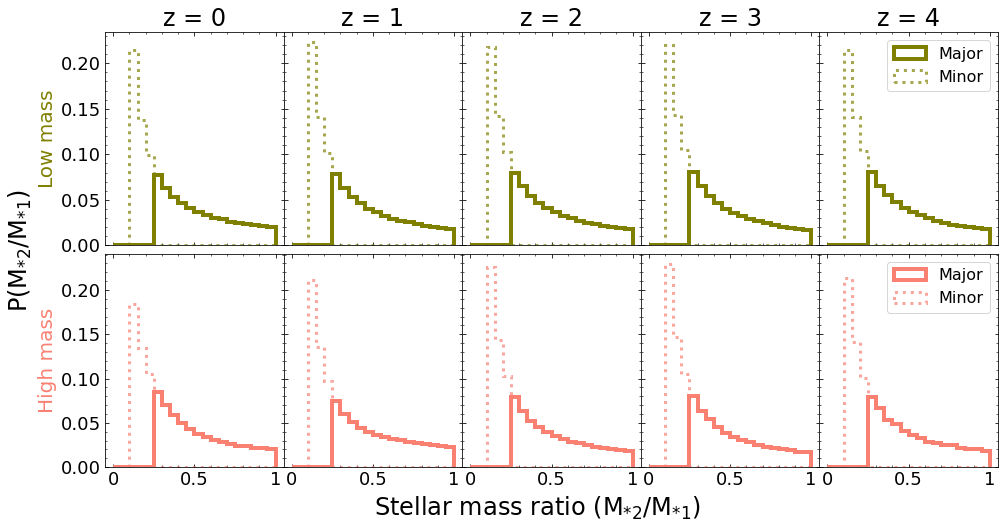
\includegraphics[width=\textwidth]{smrdist_1000.png}
    \caption{Stellar mass ratio distribution of all dwarf (top) and massive (bottom) pairs. Major pairs (solid lines) are defined as pairs with mass ratio $\ms{2}/\ms{1} > 1/4$, while minor pairs (dotted lines) are defined as pairs with stellar mass ratio $1/10<\ms{2}/\ms{1}<1/4$. Overall, the stellar mass ratio distribution of major and minor pairs of dwarf and massive galaxies show little evolution from $z=4$ (right) to $z=0$ (left). 
    Major pairs make up $51-55\%$ of the full sample of pairs at every redshift for both dwarf and massive pairs.}
    \label{fig:massratio}
  \end{figure*}

% end method plots %  
%%%%%%%%%%%%%%%%%%%%%%
  
% \begin{table*}[htb]
%   \centering
%     \begin{tabular}{lcc}
%      & Dwarf Pairs & Massive Pairs \\\hline\hline
%     % Group Mass & $8\times10^{10} < \rm M_g < 5\times10^{11} M_\odot$ & $1\times10^{12} < \rm M_g < 4\times10^{12} M_\odot$  \\
%     % Subhalo Max Mass &  &  \\
%     % Subhalo Current Mass & $>1\times10^{10} \Msun$ & $> 5\times10^{11} \Msun$ \\
%     Primary &$1\times10^{8} < \msam < 5\times10^{9} \Msun$ & $5\times10^{9} < \msam < 1\times10^{11} \Msun$\\\hline
%     \end{tabular}
%     \caption{\label{table:mass}Selection criteria for dwarf and massive pairs.}
%     \end{table*}

% equivalent snapshot table
% \begin{table*}[tbp]
%   \centering
%   \begin{tabular}{l|cc|cccc} % increase this to 7 columns
%     \hline \hline
%    & {Snapshot} & {Number of primaries} & {Number of pairs}\\
%    & \ill & \tng  & \illd & \illh & \tngd & \tngh \\ 
%   \hline
%   z = 0   &   135  &   99   & $11431.5_{-24.42}^{68.38}$ & $12650.0_{-25.84}^{46.84}$ & $13255.0_{-32.60}^{56.72}$ & $12035.0_{-69.24}^{20.36}$\\
%   z = 1   &   85   &   50   &  $14769.0_{-30.24}^{47.28}$ & $16568.0_{-32.20}^{69.60}$ & $17445.5_{-40.86}^{51.90}$ & $15946.5_{-59.38}^{39.22}$ \\
%   z = 2   &   68   &   33   &  $12602.5_{-31.98}^{45.94}$ & $14174.0_{-12.48}^{62.32}$ & $15413.5_{-34.62}^{28.86}$ & $14334.0_{-29.44}^{45.24}$ \\
%   z = 3   &   60   &   25   &     $8533.5_{-54.50}^{39.46}$ & $9390.0_{-63.40}^{41.32}$ & $10901.0_{-44.64}^{46.56}$ & $10106.5_{-47.90}^{39.74}$  \\
%   % z = 3.7   &   54   &   21   \\
%   \hline \hline
%   \end{tabular}
%   \caption{\label{tab:equiv-snapshot} The snapshot number of the original \ill\ and the \tng\ simulations at redshifts $z=0-3$, as well as the median number dwarf (massive) primaries that were selected with $1\times 10^{8} < \msam < 5\times 10^{9} \rm M_\odot$ ($5\times 10^{9} < \msam < 1\times 10^{11} \rm M_\odot$) in XX abundance matching realizations. \kc{fill in with numbers after doing more realizations} \kc{include takeaway}}
%   \end{table*}

% % %%%%%%%%%%%%%%%%%%%%%%%%%%%%%%%%%%%
% % %%%%%%%%%%%%%%%%%%%%%%%%%%%%%%%%%%%
% % %%%%%%%%%%%%%%%%%%%%%%%%%%%%%%%%%%%
% %
\section{Results}
We collect dwarf pairs and massive pairs at all snapshots from the TNG100-1 simulation. 
We analyze the occurrence rate and kinematic behavior of the pairs across cosmic time, and .... 

In Sec.~\ref{sec:results-defs}, we define each of the parameters we will be considering and provide a brief explanation of how we calculate the data we show \kc{oof help}.
In Sec.~\ref{sec:results-frac}, we show the redshift evolution of the fraction of primaries with a major or minor companion (the ``pair fraction") and compare dwarf pairs and massive pairs.
In Sec.~\ref{sec:results-kinematics}, we look at the redshift evolution of the separations and relative velocities between primary and secondary halos of each pair. % need to specify this is snapshot by snapshot?
In Sec.~\ref{sec:results-scaled}, we compare the ``scaled" separations and velocities of dwarf and massive pairs.

%%%%%%%%%%%%%%%%%%%%%   
% Definitions start %
\subsection{Definitions} \label{sec:results-defs}
    The pair sample consists of 1000 sets of pairs at each snapshot, each set representing a different realization of the abundance matching prescription. 
    In each of the following plots, the median and a percentile spread each value are calculated by finding the median from each of the 1000 AM realizations, and taking the median and spread of that set of median values.
    
    \begin{itemize}
        \item[-] \textbf{Pair fractions:} the major pair fraction is the ratio of the number of major pairs to the total number of primaries (isolated + paired). 
        The minor pair fraction is defined in a similar way. 

        \item[-] \textbf{Separations:} pair separations are defined as the relative separation between the primary and secondary of each pair. 
        Pair separations are computed in physical units, not comoving. 
        
        \item[-] \textbf{Velocities:} relative velocities are defined as the relative velocity difference between the primary and secondary of each pair. 
        This can be interpreted as the velocity of a secondary with respect to a stationary primary. 
        Relative velocities are computed in physical $\kms$. 
        
        \item[-] \textbf{Scaled velocities and separations:} scaled 
        
        \item data presented (median def and spread)


    \end{itemize}

% Definitions end %
%%%%%%%%%%%%%%%%%%% 


%%%%%%%%%%%%%%%%%%%%%%%%%
% Pair fraction section %
\subsection{Pair fraction}\label{sec:results-frac}
    % intro to pair frac plot
The pair fraction is defined here as the fraction of identified dwarf or massive primaries with a major or minor companion (see Sec.~\ref{sec:methods-crit} for more info on selection criteria for major and minor pairs). 
Fig.~\ref{fig:pairratio} shows the pair fractions calculated for massive and dwarf pairs (including both major and minor pairs separately) as a function of time for $z=0-4$. 

    % differences between massive and dwarf pairs? 
The dwarf pair fraction evolves distinctly from that of massive pairs.
Both major and minor dwarf pair fractions start at their minima at $z=0$, and increase by about 200\% by $z\sim2-2.5$, at which point the pair fractions level off and remain constant from $z=3-4$. 
The major and minor pair fractions for massive pairs evolve similarly, starting at their maxima at $z=0$, then abruptly declining to $z\sim0.25$, before remaining approximately constant from $z=1-4$ %(see Table~\ref{table:vals} for more precise values of the pair fractions). 

    % difference panels
The bottom panel of Fig.~\ref{fig:pairratio} shows the dwarf pair fraction subtracted from the massive pair fraction (labelled ``$\rm M-D$"). 
The pair fraction difference reaches a maximum at $z=0$ for both major and minor pairs, and declines to $z\sim2-2.5$ at which point the difference levels out close to 0. 

    % differences between major and minor pairs? 
The median pair fraction for minor pairs (for both dwarf and massive galaxies) is less than that of major pairs of the same mass range at all redshifts. This is due to the lower stellar mass ratio limit we put on our pairs. 
Expanding the mass ratio criteria of our minor pair sample to include stellar mass ratios between 1/10-1/100 in our minor pair sample increases the fraction of minor pairs by a factor of $>2$ for massive pairs and between $~1.5-2x$ for dwarf pairs. \kc{are there any additional takeaways from this? }

    % what do we learn from this? what are the takeaways? where do we discuss this in more detail?
Overall, these results show that massive and dwarf pair counts evolve differently, particularly at very low redshift despite the pair fractions being roughly equal at higher z. 
These differences could be a result of the different formation mechanisms at play in the evolution of the systems at these two different mass scales, or alternatively, from differences in satellite dynamics between dwarf and massive systems (see Sec.~\ref{sec:results-kinematics}). 
The implications for the difference in the evolution of pair fractions for dwarf and massive pairs across time is discussed in detail in Sec.~\ref{sec:discussion}.

    % pair fraction plot
\label{sec:results}
\begin{figure*}[htp]
  \centering
  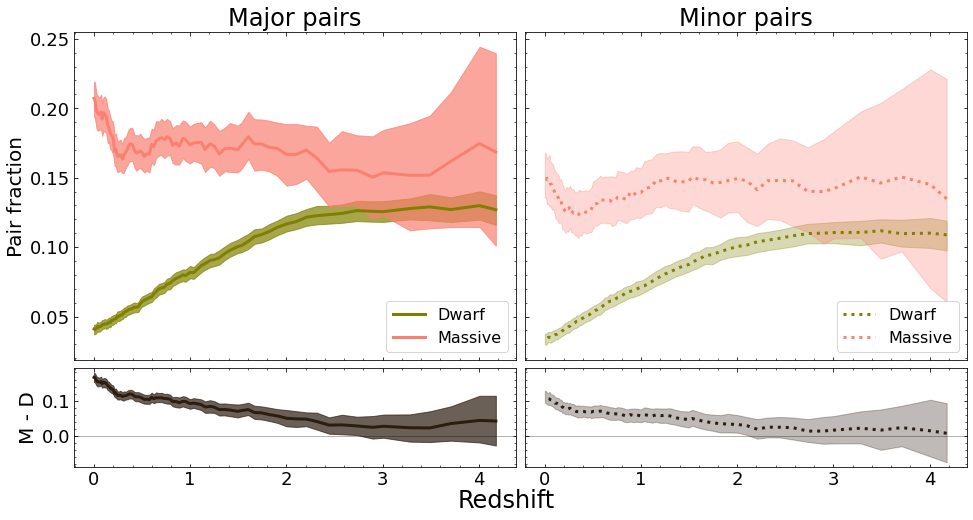
\includegraphics[width=\textwidth]{pairfrac_1000.png}
  \caption{
    % Top plots ~
    (Top) Median pair fraction, defined as the fraction of dwarf or massive primaries with a major (left) or minor (right) companion by stellar mass (see Sec.~\ref{sec:methods-pairs}). 
    Shaded areas show the 1-99 percentile range of the median from 1000 abundance matching realizations. 
      % massive pairs
    The massive pair fraction (pink) remains approximately constant for $z>1$, with an average pair fraction of 0.16-0.17 for major pairs and 0.14-0.15 for minor pairs. Between $z=0.25$ and $z=0$, the massive major pair fraction increases to 0.207, while the minor pair fraction increases to 0.152.
      % dwarf pairs
    Dwarf pair fractions, shown in green, are approximately constant from $z=3-4$, then declines monotonically to $z=0$. The major pair fraction is $0.041$ at $z=0$ and $0.126$ at $z=3$, while the minor pair fractions are $0.034$ and $0.111$ at $z=0$ and $z=3$, respectively. 
    % Bottom plots ~
    (Bottom) The median subtracted (massive - dwarf) pair fraction difference, with the shaded $1$-$99$ percentile range from 1000 abundance matching realizations. The pair fraction difference increases with decreasing redshift, peaking at $z=0$ with a difference of 0.166 for major pairs and 0.111 for minor pairs. This shows that the redshift evolution of the pair fractions of massive pairs and dwarf pairs proceed differently, particularly in the low redshift regime.}
  \label{fig:pairratio}
\end{figure*}
% end pair fraction 
%%%%%%%%%%%%%%%%%%%%%%%%%

%%%%%%%%%%%%%%%%%%%%%%
% Kinematics section %
\subsection{Kinematic evolution}\label{sec:results-kinematics}
At each individual snapshot, we find the instantaneous separation and relative velocity of the primary and secondary halo of every pair that was selected in the snapshot. 
This is done separately for all 1000 different abundance matching realizations at each snapshot, as described in Sec.~\ref{sec:methods-am}, then we explore the properties of the set of median separations and velocities for each realization. 
In this section, we compute the median relative separations and velocities of all 1000 realizations of dwarf and massive pairs, and show their behavior as a function of redshift.
We separate the population of pairs into "major" and "minor" pairs (as defined in Sec.~\ref{sec:methods-pairs}) to show how the stellar mass ratio between the primary and secondary may affect the kinematics. 


% separations %
    \subsubsection{Separations}
    %% text on separation vs. redshift plot
    %% intro to separations & bulk results
    We calculate the median relative separations between the primary and secondary halos of the pairs identified in our dwarf pair sample and massive pair sample. 
    We split the results by the stellar mass ratio of each pair, dividing the sample into "major" pairs and minor pairs, which allows us to compare the behavior of different mass ratio systems individually in the dwarf and massive mass range.
    Our results are collected in Fig.~\ref{fig:sep}, which shows the redshift evolution of the median relative separations for dwarf pairs and massive pairs. 
    
    %% the behavior of massive and dwarf pairs
    We show that the median relative separations between the primary and secondary of both dwarf and massive pairs increases with decreasing redshift, regardless of pair type. 
    A combination of physical mechanisms is likely spurring the increase in median pair separations at low $z$. 
    For example, high $z$, low separation pairs may undergo mergers at earlier times, removing them from the sample at later snapshots, thus increasing the median separation over time. 
    Alternatively, mass accretion, from the cosmic web and/or from mergers, causes dark matter halos to become both more massive and more extended as $z\to0$. 
    Thus, the growth of structure that is expected in $\Lambda$CDM could naturally lead to an increase in typical pair separations at low $z$.
    We explore the relationship between halo growth and relative pair separations in Sec.~\ref{sec:results-scaled}.
    
    %% the DIFFERENCE between dwarf and massive pairs
    Dwarf and massive pairs exhibit similar relative separation trends as a function of time, however, the scale of the typical relative separations of pairs in our sample is set by the mass halo of the primary.
    Dwarf pairs and massive pairs have a relative separation difference of $\sim150\kpc$ at $z=0$, and a difference of $\sim40$ at $z=4$.   
    This is expected, as more massive halos have larger spheres of influence and more substructure. 
    \kc{maybe move this sentence to discussion:}But, the difference between dwarf and massive pair relative separation ranges, and their evolution over time begs the question: what does this mean for observational pair selection criteria at different mass scales and at different redshifts? 
    We leave the discussion of the implications our relative separation results on pair selection criteria for Sec.~\ref{sec:discussion}. 
    
    %% the difference between major and minor pairs
    In addition, Fig.~\ref{fig:sep} shows the median subtracted difference between the relative separations calculated for major pairs and minor pairs of both mass type. 
    There is a small offset in the median separations of major and minor dwarf pairs (between $10-25\,\kpc$ from  $z=0-1$ and approximately $5\,\kpc$ from $z=1-4$), and a larger median separation offset for major and minor massive pairs (between $25-100\,\kpc$ from  $z=0-1$ and approximately $10-40\,\kpc$ from $z=1-4$). 
    The major-minor offset is likely a result of more major pairs merging more quickly (thus at earlier times and higher $z$) due to the increased effect of dynamical friction, thus leading to a population of low relative separation minor pairs that have yet to merge.  

    %% separation plots
    \begin{figure*}[htp]
      \centering
      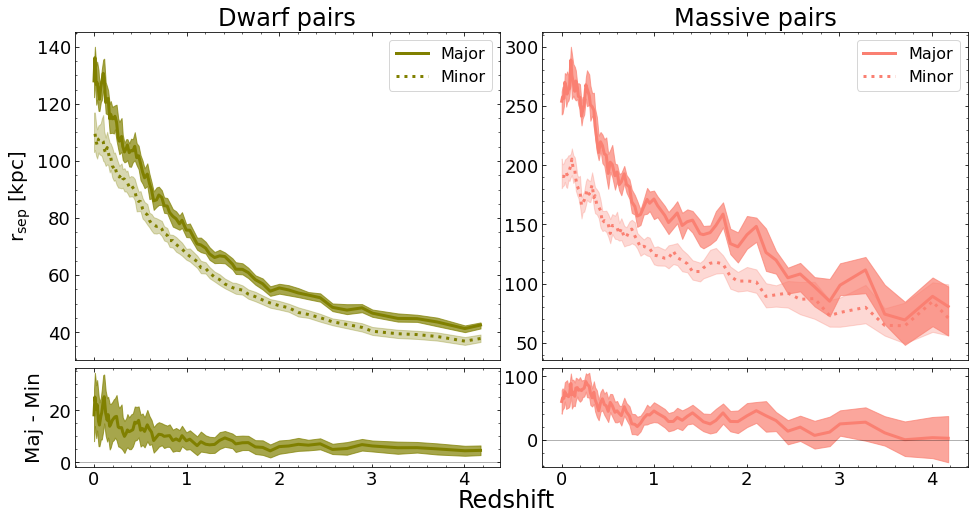
\includegraphics[width=\textwidth]{sep_1000.png}
      \caption{(Top) Median physical separation in kpc between the primary and secondary halos of dwarf pairs (left) and massive pairs (right) as a function of redshift. 
      Shaded areas show the 1-99\% percentile range of the median from 1000 abundance matching realizations. 
      Major pairs are shown in solid lines, and minor pairs are depicted with dashed lines.
      In general, for both dwarf pairs and massive pairs, the average physical separation of the two halos in a pair increases for as the redshift decreases from $z=4\to0$. 
      % Dwarf pairs
      The typical separation between major (minor) dwarf pairs increases from $42(38)\,\kpc$ at $z=4$ to a peak of $128(109)\,\kpc$ at $z=0$.
      % Massive Pairs
      The separation between major (minor) massive pairs likewise increases from $81(71)\,\kpc$ at $z=4$ to $288(205)\,\kpc$ at  $z=0$.
      % Difference plots
      (Bottom) The median difference and 1-99\% range (as above) between the median separation of major pairs and minor pairs.
      At dwarf mass scales, minor companions tend to be $\sim10-20\kpc$ closer to their primary than major companions, while minor massive pairs have a relative separation that is $10-50\kpc$ less than major pairs.
        }
      \label{fig:sep}
    \end{figure*}

% velocities %
    \subsubsection{Relative Velocities}
    %% text on velocity vs. redshift plot
    %% intro to velocity & bulk results
    In addition to the separations between the primary and secondary halos of our pair sample, we also calculate the median relative velocity between the halos of each pair.
    Once again we split the results into "major" and "minor" pairs for both the dwarf and massive pair sample to get a better understanding of the impact of the mass of the secondary. 
    In Fig.~\ref{fig:vel}, we show the median relative velocity between the primary and secondary halos of dwarf and massive pairs as a function of redshift. 
    Note that these relative velocities are calculated from the instantaneous velocity of the halos at the snapshot the pair is in (see Sec.~\ref{sec:methods} for more details about our velocity calculations).
    
    %% the behavior of massive and dwarf pairs
    We find that the median relative velocity between a pair's primary and secondary halo decreases towards lower redshift, regardless of pair type.
    The median velocity of a major dwarf pair decreases linearly from $130$ at $z=4$ to $70\,\kms$ at $z=0$. Likewise, the median velocity for major massive pairs decreases from $260$ at $z=4$ to $170\,\kms$ at $z=0$, though with more spread at high $z$.
    As the circular velocity of a secondary object about the primary is inversely proportional to the radius, it is not surprising to find a decrease in the relative velocity for pairs at lower redshift due to the expansion of the universe/decrease in concentration/increase in the virial radius of the halo as $z\to0$. \kc{citation needed}
    See Sec.~\ref{sec:results-scaled} for more details.
    
    %% the DIFFERENCE between dwarf and massive pairs
    As in the case of relative separations of pairs, dwarf and massive pairs show a similar evolutionary trend in relative velocity as a function of redshift, though at different scales determined by the mass of the primary.
    Massive pairs have a median relative velocity $\sim100\kms$ larger than dwarf pairs at $z=0$, and $\sim140\kms$ at $z=4$. \kc{see comment}
    %This is also not particularly surprising, since the circular velocity prop to $( M/r)^1/2,$, and massive primaries may be >10x as massive as dwarf primaries, while the separation between a massive primary and it's secondary will only be 2x further than a dwarf pair.

    %% the difference between major and minor pairs
    Fig.~\ref{fig:vel} also includes a panel showing the subtracted median difference at each snapshot of the minor pair from the major pair. Unlike the relative separation, the relative velocities do not have a strong dependence on the secondary mass. 
    Since minor pairs typically have slightly higher velocities than their major pair counterparts, this difference is usually $<0$. The offsets between the relative velocities of dwarf major and minor pairs is between $0-5\,\kms$, and between $0-25\,\kms$ for massive major and minor pairs. \kc{see comment} %does it make sense that minor pairs are faster?
    
    %% velocity plots 
    \begin{figure*}[htp]
      \centering
      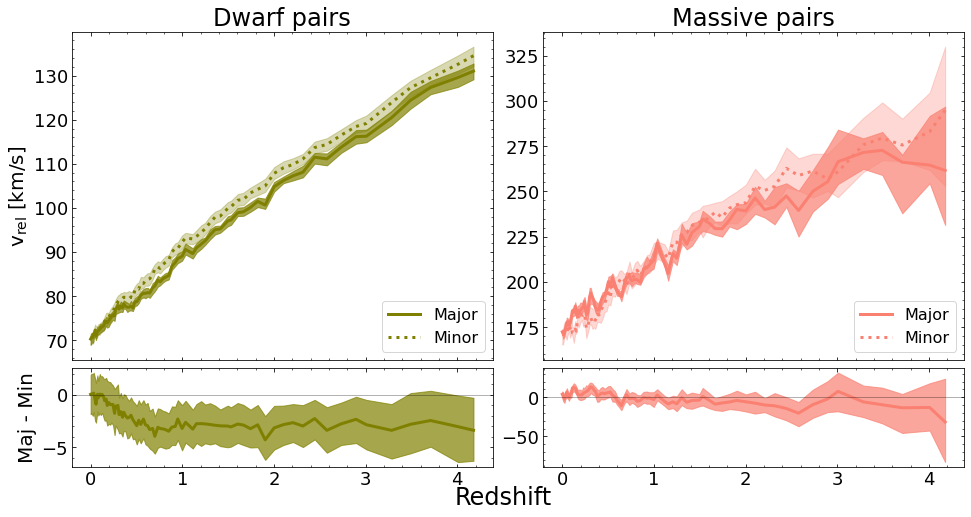
\includegraphics[width=\textwidth]{vel_1000.png}
      \caption{
        (Top) Median relative velocity (in \kms) between the primary and secondary halos of dwarf pairs (left) and massive pairs (right) as a function of redshift. 
        Shaded areas show the 1-99 percentile range of the median from 1000 abundance matching realizations. 
        The overall behavior of the redshift evolution of pair relative velocities is nearly identical for dwarf and massive pairs.
        As the redshift decreases from $z=4$ to $z=0$, the average relative velocity of a pair decreases for both dwarf and massive pairs.
        % brief describe
        The median relative velocity of a dwarf pair (major or minor) is $70\,\kms$ at $z=0$ and $133\,\kms$ at $z=4$, and of a massive pair is $170\,\kms$ at $z=0$ and $260\,\kms$ at $z=4$ ($295\,\kms$ for a minor pair at $z=4$). 
        % Difference plot
        (Bottom) The median relative velocity difference between major and minor pairs ("Maj - Min"), and 1-99\% shaded region.
        There is little difference between the relative velocity of major and minor dwarf pairs (bottom left), with minor pairs having a relative velocity of $0-5\,\kms$ higher than major pairs. 
        Massive pair types (bottom right) also have little velocity difference at low redshift, although minor pairs have a relative velocity between $1-20\,\kms$ faster than major pairs at higher redshift ($z>\sim 2.5$).
        }
      \label{fig:vel}
    \end{figure*}

% scaled results %
\subsection{Scaled Kinematics}\label{sec:results-scaled}
%% intro to scaled kin. evolution & bulk results
In Sec.~\ref{sec:results-kinematics}, we show that the separations and relative velocities of dwarf and massive pairs evolve similarly as a function of redshift. 
However, the magnitude of pair separations and velocities are set by the mass scale of the pair. 
For example, a dwarf pair at $z=0$ has a median relative velocity of $70\kms$, while a massive pair will have a median velocity of $175\kms$ at $z=0$.

To explore the impact of halo growth and mass scale the kinematics pairs, we study the relative separation of a primary and secondary halo scaled by the virial radius of the FoF group (\scsep), and the relative velocity divided by the circular speed of the group at the virial radius (\scvel).     
In Fig.~\ref{fig:scaled}, we show the median scaled separation and scaled velocity for dwarf and massive major pairs as a function of time. 
Minor pairs show the same trends, so we've omitted them here for brevity.

%% the behavior of massive and dwarf pairs
Overall, the median scaled separation of dwarf pairs and massive pairs do not evolve significantly differently from $z=4\to0$.
In fact, the median separation of halos in a pair is smaller than the group virial radius for at $z<2.5$, but is larger than the virial radius at $z>2.5$.
%maybe not bound at high z, though could become bound by low z by mass accretion ? 
Dwarf pairs tend to have slightly larger separations relative to their virial radius than massive pairs at almost all redshifts, though the spread of median scaled separations is large for massive pairs at $z>2$. 

The median scaled velocities of dwarf pairs and massive pairs increase at lower redshift (see right panel of Fig.~\ref{fig:scaled}). In fact, dwarf and massive pairs evolve almost identically for $z=0-4$, and thus, the redshift evolution of a pair at either of these mass scales is independent of the total mass of the system. 
We also find that pairs at $z<0.5$ have relative velocities in excess of their virial velocity, but are smaller than the virial velocity for $z=0.5-4$.
 
%% distributions of scaled kinematics
In Fig.~\ref{fig:scaled-dist}, we show the distribution of scaled separations and velocities at redshifts $z=0,1,2,3,4$. 
The distributions show roughly equivalent shape and extent for both dwarf and massive scaled kinematics, and do not vary significantly with redshift. 
scaled separation, and velocity both, this is due to the growth of halos, so while the separation increases, the halo radius also increases.
% behavior of massive vs. dwarf 
Overall, our results imply that there is little to no mass dependence on the redshift evolution of pair velocities, though pair separations seem to have a weak dependence on the total system mass. 

%% scaled evolution plot
\begin{figure*}[htp]
  \centering
  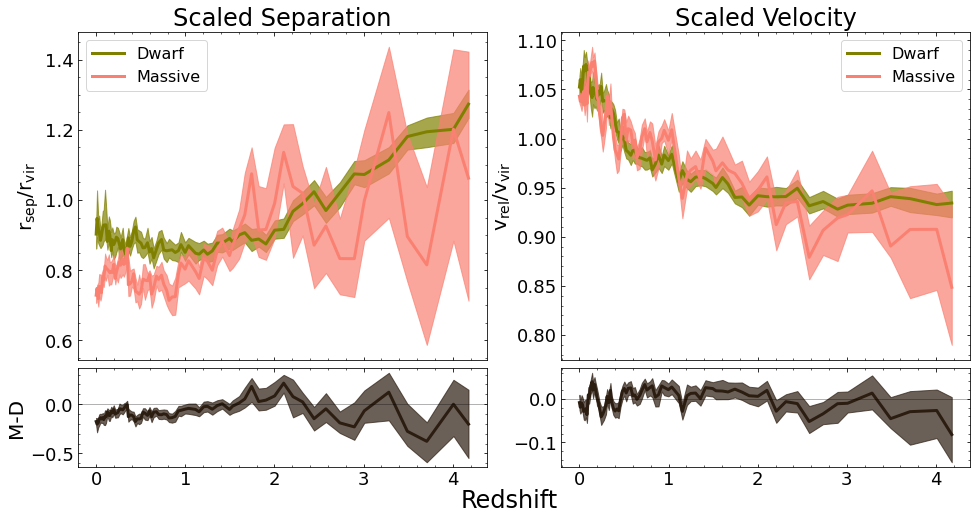
\includegraphics[width=\textwidth]{scaledcombo_1000.png}
  \caption{ \label{fig:scaled}
      %  Left
      (Left) Median scaled separation as a function of redshift (see Sec.~\ref{sec:methods} for the definitions of scaled separation and velocity). All shaded regions show $X-XX\%$ percentile spread from 1000 abundance matching realizations. 
      % any overall trends?
      At $z>2$, a majority of all pair types have separations greater than the group virial radius, while at $z<2$, a majority of pairs have smaller separations.  
      Massive major pairs at low redshift tend to have slight smaller scaled separations than dwarfs at $z<\sim2$, but vary significantly at higher redshifts. 
      % Right 
      (Right) Median scaled velocity as a function of redshift.
      % any overall trends?
      All pairs show a peak in scaled velocity around $z=0$. From $z=0-0.5$, a majority of both dwarf and massive pairs have relative velocities larger than the circular velocity of their group at the virial radius. At $z>0.5$, however, the majority of pairs have $v_{rel}<v_{vir}$. The scaled velocity evolves nearly identically for dwarf and massive pairs.
      % Bottom 
      (Bottom) The scaled separation/velocity of dwarf major pairs subtracted from that of massive major pairs, indicated by ``M-D".
      The scaled separation difference shows small differences between the dwarf and massive population, with dwarf pairs having slightly higher scaled separation for $z<1$. The scaled velocity difference is $\sim0$ at all redshifts.
      Minor pairs (not shown here) follow the same trends as major pairs in both the massive and dwarf regime.}
\end{figure*}

%% scaled distribution plot
\begin{figure*}[htp]
  \centering
  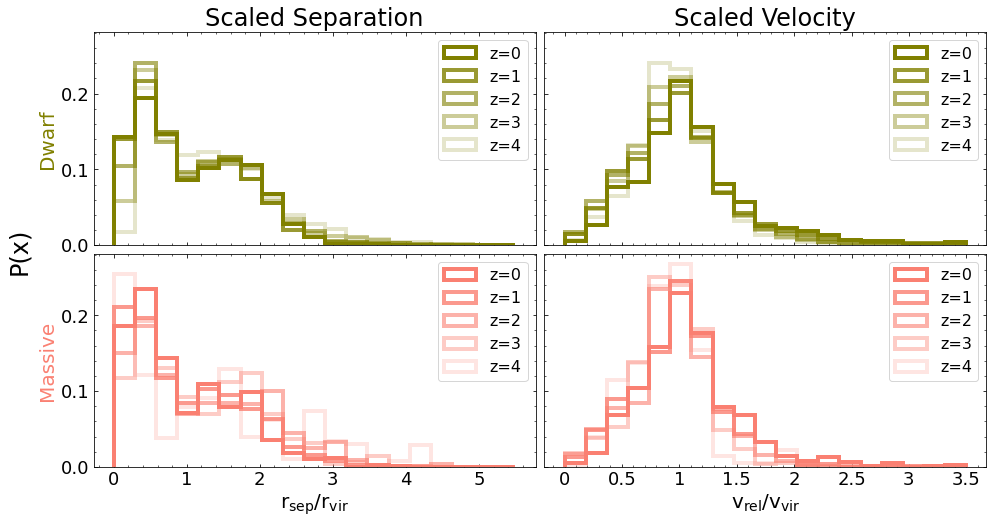
\includegraphics[width=\textwidth]{scaledcombodist_1000.png}
  \caption{
      Scaled separation distribution (left) and scaled velocity distribution (right) at $z=0,1,2,3$, and $4$, normalized by the total number of pairs at the corresponding redshift. 
      % the point? what am I trying to get across
      The first thing to note is that there is relatively little redshift-dependent change in the overall shape and extent of each distribution, and thus the scaled quantities are only loosely independent of redshift. 
      Additionally, the shape and extent of the dwarf pair (top) and the massive pair (bottom) distributions are nearly identical, thus the scaled quantities are also independent of the halo mass scale. Thus, the kinematics of dwarf pairs and massive pairs evolve roughly equivalently when normalizing by the halo mass.
      Unscaled versions of this plot are discussed in Sec.~\ref{sec:discussion}.
  }
  \label{fig:scaled-dist}
\end{figure*} 

% end kinematics
%%%%%%%%%%%%%%%%%%%%%%

%%%%%%%%%%%%%%%%%%%%%%
% Discussion section %
\pagebreak
\section{Discussion}\label{sec:discussion}

\subsection{Comparison to previous works/literature}
\begin{itemize}
    \item our pairs are not projected dist, so represent set of maximum seps/vels possible
    \item compare to Synder 2022+
    \item compare to Lotz and Rodriguez Gomez 
\end{itemize}

\subsection{Implications for differences in massive and dwarf pair evolution?}


\subsection{Implications for observational pair definitions}
    \begin{itemize}
        \item examples of typical pair selection criteria
        \item Sep distribution explanation
        \item Vel. distribution ex.
        \item quantify \% of pairs > current cuts 
        
    \end{itemize}
    
\subsection{Low separation implications for JWST and other wide and deep surveys}

\subsection{Limitations of our methods}
\pagebreak
% Mean separation fig. -- 

% Separation dist fig. -- The number of widely separated pairs at low redshift is much greater than at high redshift, so these pairs either form late, or move apart from each other. 




% Also note than many of the close pairs at high z may merge by $z=0$.





% \subsection{Massive pairs vs. Dwarf pairs}
% Pair ratio fig. -- The vast difference between the dwarf and massive pair fractions suggests \todo{XX - that pairs at different mass scales evolve differently ? Thus, can't just assume a massive pair fraction for a lower mass regime} 

% \subsection{Dwarf and massive pair kinematic differences}

% \subsection{Comparison to literature}

% \subsection{Implications for observations}

% \subsection{Implications for observational pair selection criteria}
% %% text on separation distribution plot
% Fig.~\ref{fig:sep-dist} shows the full distribution of separations for major and minor dwarf and massive pairs at $z=\{0,1,2,3,4\}$, and includes all 1000 AM realizations. 
% For reference, the median at each corresponding redshift from Fig.~\ref{fig:sep} (that is, the median of the medians of each realization) are shown in light black vertical lines.
% Each plot is normalized such that the area under an individual curve is 1.
%     % the redshift evolution
% All pair types (dwarf and massive, major and minor) have narrow distributions that pile up around 0 $\kpc$ at $z=4$, but the distributions become more and more broad as $z\to0$ (note that only pairs with separations $>10\kpc$ are included in this analysis, see Sec.~\ref{sec:methods-crit-pairs}).
% \linebreak
% The distribution profiles are similar when the scale of the x-axis for massive pair separations is twice that of the dwarf pairs. 
% Pair separations at $z=0$ tend to primarily fall between $10-\sim400\,\kpc$ for dwarf pairs and   between $10-\sim1000\,\kpc$ for massive pairs. 
% At $z=4$, these ranges decrease to $10-150\,\kpc$ for dwarf pairs and $10-300\,\kpc$ for massive pairs. 
%     % comparing major and minor
% Major and minor pairs (both dwarf pairs and massive pairs) have roughly equivalent distributions, though the distribution of minor pairs with low separations is slightly higher than the major pairs. Thus, secondary halo of minor pairs tend to live slightly closer to their primaries than the  major secondaries.

% \begin{figure*}[htp]
%   \centering
%   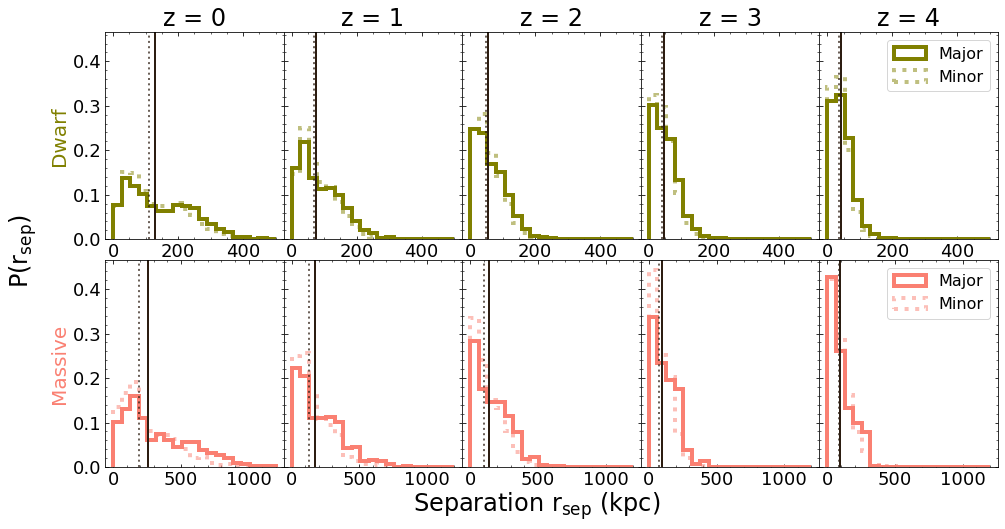
\includegraphics[width=\textwidth]{sepdist_1000.png}
%   \caption{Normalized physical separation distribution for dwarf (top) and massive (bottom) pairs from $z=0$ (left) to $z=4$ (right). Major pairs are shown as solid lines, while minor pairs are dotted. The median separation of each pair type from the previous plot is shown in solid (major) and dotted (minor) vertical black lines. 
%   At higher redshift $z=3-4$, a large fraction of both dwarf and massive pairs have low separations ($<$ 125 \& 250 $\kpc$ respectively). However, at low redshift, the separation distribution tends to spread out more evenly across a large range of separations, thus increasing the median.
%     }
%   \label{fig:sep-dist}
% \end{figure*}

% \begin{figure*}[htp]
%   \centering
%   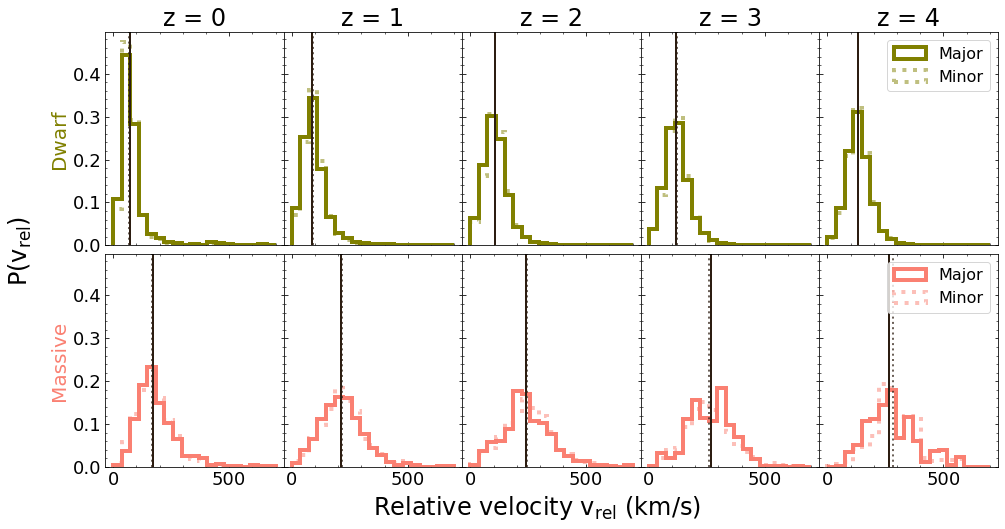
\includegraphics[width=\textwidth]{veldist_1000.png}
%   \caption{
%   Normalized distribution of relative velocities between primary and secondary halos for dwarf (top) and massive (bottom) pairs from $z=0$ (left) to $z=4$ (right). Major pairs are shown as solid lines, while minor pairs are dotted. The median relative velocity of each pair type from Fig.~\ref{fig:vel} is shown in solid (major) and dotted (minor) vertical black lines. 
%   %
%   The distribution of relative velocities for dwarf and massive pairs move to slightly lower velocities at lower redshifts. 
%   At $z=0$, typical dwarf pair relative velocities are $0-200\,\kms$, while at $z=4$ they are $0-300\,\kms$. 
%   Massive pairs typically have relative velocities between $0-300\,\kms$ at z=0 and $0-400\,\kms$ at $z=4$.
%   The distribution of velocities for major and minor pairs is roughly equivalent within each mass range. 
%     }
%   \label{fig:vel-dist}
% \end{figure*}

% %% text on velocity distribution plot
% \kc{left off here\~}
% Fig.~\ref{fig:vel-dist}

%%%%%%%%%%%%%%%%%%%%%%


%%%%%%%%%%%%%%%%%%%%%%%%%%%%%%%%%%%
\pagebreak
\section{Summary and Conclusions}\label{sec:summary}
\begin{itemize}
    \item What we did 
    \item Main findings:
        \begin{itemize}
            \item pair fractions
            \item separations
            \item velocities
            \item scaled values
        \end{itemize}
    \item Main takeaways: (maybe include these within main findings bullets~)
        \begin{itemize}
            \item lit comp.
            \item dwarfs not equal massives 
            \item JWST imps.
        \end{itemize}
    \item Future work
\end{itemize}

% Findings:
% \begin{itemize}
%     \item Pair fraction for dwarfs and massives does not proceed identically throughout cosmic time. Opposite behavior at low z. 
%     \item Median pair separations increase and relative velocities decrease from high to low redshift. 
% \end{itemize}

%%%%%%%%%%%%%%%%%%%%%%%%
%%%%%%%%%%%%%%%%%%%%%%%%

\bibliography{refs}{}
\bibliographystyle{aasjournal}

\end{document}
